\documentclass[a4paper,12pt]{article}
\usepackage{czech}
\usepackage[utf8]{inputenc}
\usepackage{a4wide}
\usepackage[dvipdfm]{graphicx}
\usepackage{graphics}
\usepackage{indentfirst}
\usepackage{fancyhdr}
\usepackage{setspace}
\usepackage{amsmath}
\usepackage{amssymb}
\usepackage{epsfig}

%%\usepackage{nopageno}
%%\usepackage{txfonts}
\usepackage[usenames]{color}

\begin{document}
\section{Úkol}
\noindent
\begin{enumerate}
	\item Změřte anodové charakeristiky triody EC(C)83. Mřížkové napětí $U_g$ měňte od 0 do -2 V 
    po krocích 0.5 V. Při měření nepřekračujte maximální anodovou ztrátu $P_a = 0.2 \mbox{W}$.
    Anodové napětí zvyšujte maximálně do 120 V.
	\item Změřte závislost zesílení $A = U_{vyst}/U_{vst}$ (poměr výstupního napětí ke vstupnímu) 
    triodového zesilovače na frekvenci pro $U_g = -1 \mbox{V}, U_a = 120 \mbox{V}, R_a=10^5 \Omega$ 
    a $R_a = 5\cdot 10^3 \Omega, U_{vst} = 0.3 \mbox{V}$ ve frekvenčním rozsahu 30 Hz - 100 kHz.
	\item Změřte závislost zesílení $A$ na velikosti anodového odporu pro $U_a = 120 \mbox{V}$ v
    rozsahu $R_a = 5 \cdot 10^3 - 10^5 \Omega. U_g = -1 \mbox{V}$ při $f = 1 \mbox{kHz}, U_{vst}=0.3 \mbox{V}$.
	\item Anodové charakteristiky zpracujte graficky. V grafu vyznačte oblast, kde byla překročena 
    anodová ztráta $P_a = 0.2 \mbox{W}.$ Zakreslete rovněž zatěžovací přímky pro obě hodnoty anadového 
    odporu $R_a$ z úkolu 2. Určete odpovídající pracovní body a stanovte příslušné hodnoty zesílení a průběh 
    frekvenčních charakteristik.
\end{enumerate}

\section{Teorie}

\subsection{Trioda}
Trioda je druh elektronky skládající se z dvou elektrod a mřížky. Jedná se o nejednodušší typ zesilovače, 
kdy se velikost anodového proudu ovlivňuje napětím na mřížce. 

\subsection{Měření charakteristik triod}
Charakteristiky triody se měří při zapojení dle obrázku 1 z \cite{text}, kde anodové napětí $U_a$ odečteme 
z voltmetru V, anodový proud $I_A$ z miliapérmetru mA a napětí na mřížce $U_g$ z voltmetru V$_1$.

\subsection{Měření zesílení zesilovače}
Zesílení $A$ je definováno vztahem

\begin{eqnarray}
A = \frac{U_vyst}{U_vst},
\label{A}
\end{eqnarray}

kde $U_vyst$ je výstupní napětí a $U_vst$ napětí vstupní.

Měří se v zapojení dle obrázku 2 z \cite{text}, kde tečky s písmeny značí jendotlivé uzly triody.

\subsection{Chyby}
V průběhu celého měření byly použity pouze analogová měřidla. Chyba měření je proto dána jejich třídou přesnosti a rozsahem, 
na kterém bylo měřeno. Abolutní chyba je dána vztahem 
\begin{eqnarray}
\sigma = \frac{R\cdot k}{100},
\end{eqnarray}
kde $R$ je rozsah a $k$ třída přesnosti.

Dále vystupuje nepříma chyba měření u zesílení $A$, jejíž relativní chybu získáme součtem relativních chyb z voltmétrů.

Třídy přesnosti jednotlivých přístrojů byly:
\begin{enumerate}
    \item Ampérmetr úkol 1 - 1
    \item Voltmetr úkol 1 - 0.5
    \item Voltmetr na generátoru $U_{vst}$ - 1.5
    \item Voltmetr $U_{vyst}$ - 1.5
\end{enumerate}


\section{Měření}

\subsection{Anodové charakteristiky}
V zapojení dle obrázku 1 z \cite{text} jsem měřil velikost anodového proudu $I_a$ na napětí $U_a$ pro různá mřížková napětí $U_g$.
Naměřené hodnoty jsou shrnuty v tabulce \ref{Ia} a zobrazeny v na obrázku \ref{g1}, kde jsou proložené pro názornost křivkou. Dále 
jsou v grafu zaneseny zatěžovací křivky pro anodové odpory z úkolu 2 a vyznačeny pracovní body triody pro tyto odpory.

\begin{table}
$$
\begin{array}{|c||c|c|c|c|c|}
\hline
U_g/\mbox{V}    &   0   &   -0.5    &   -1  &   -1.5    &   2   \\ \hline    
\hline  
U_a/\mbox{V}    &   I/\mu\mbox{A}&   I/\mu\mbox{A}  &   I/\mu\mbox{A} &   I/\mu\mbox{A} &  I/\mu\mbox{A} \\ \hline
0   &   0 \pm 0.3       &   0 \pm 0.3      &   0 \pm 0.3       &   0 \pm 0.3   &   0 \pm 0.3   \\  \hline
10  &   30 \pm 0.3  &   10\pm 0.3   &   0 \pm  0.3      &   0 \pm  0.3  &   0 \pm  0.3  \\ \hline
20  &   50 \pm 3 &   33\pm  0.3   &   0 \pm  0.3      &   0 \pm  0.3  &   0\pm  0.3   \\ \hline
30  &   110 \pm 3   &   64 \pm 1  &   5\pm  0.3   &   0 \pm  0.3  &   0 \pm  0.3  \\ \hline
40  &   220 \pm 3   &   134 \pm 1  &   18\pm  0.3   &   0 \pm  0.3  &   0 \pm  0.3  \\ \hline
50  &   335 \pm 3   &   218 \pm 1  &   37\pm  0.3   &   0 \pm  0.3  &   0 \pm  0.3  \\ \hline
60  &   455 \pm 3   &   295 \pm 3  &   64 \pm 1  &   1\pm  0.3   &   0 \pm  0.3  \\ \hline
70  &   585 \pm 3   &   410 \pm 3   &   116 \pm 1  &   7\pm  0.3   &   0 \pm  0.3  \\ \hline
80  &   680 \pm 10    &   525 \pm 3  &   178 \pm 1  &   18\pm  0.3   &   0 \pm  0.3  \\ \hline
90  &   840 \pm 10    &   620 \pm 10   &   250 \pm 3   &   37\pm  0.3   &   0  \pm  0.3 \\ \hline
100 &   1000 \pm 10    &   760 \pm 10   &   335 \pm 3  &   56 \pm 1  &   3\pm  0.3   \\ \hline
110 &   1180 \pm 10    &   920 \pm 10   &   440 \pm 3   &   96 \pm 1  &   9\pm  0.3   \\ \hline
120 &   1360 \pm 10    &   1080 \pm 10   &   565 \pm 3  &   178 \pm 1  &   19.5\pm  0.3   \\ \hline
\end{array}
$$
\caption{Tabulka vývoje anodového proudu $I_a$ v závislosti na anodovém napětí $U_a$ pro různá mřížková napětí$U_g$.}
\label{Ia}
\end{table}

\begin{figure}
% GNUPLOT: LaTeX picture with Postscript
\begingroup
  \makeatletter
  \providecommand\color[2][]{%
    \GenericError{(gnuplot) \space\space\space\@spaces}{%
      Package color not loaded in conjunction with
      terminal option `colourtext'%
    }{See the gnuplot documentation for explanation.%
    }{Either use 'blacktext' in gnuplot or load the package
      color.sty in LaTeX.}%
    \renewcommand\color[2][]{}%
  }%
  \providecommand\includegraphics[2][]{%
    \GenericError{(gnuplot) \space\space\space\@spaces}{%
      Package graphicx or graphics not loaded%
    }{See the gnuplot documentation for explanation.%
    }{The gnuplot epslatex terminal needs graphicx.sty or graphics.sty.}%
    \renewcommand\includegraphics[2][]{}%
  }%
  \providecommand\rotatebox[2]{#2}%
  \@ifundefined{ifGPcolor}{%
    \newif\ifGPcolor
    \GPcolorfalse
  }{}%
  \@ifundefined{ifGPblacktext}{%
    \newif\ifGPblacktext
    \GPblacktexttrue
  }{}%
  % define a \g@addto@macro without @ in the name:
  \let\gplgaddtomacro\g@addto@macro
  % define empty templates for all commands taking text:
  \gdef\gplbacktext{}%
  \gdef\gplfronttext{}%
  \makeatother
  \ifGPblacktext
    % no textcolor at all
    \def\colorrgb#1{}%
    \def\colorgray#1{}%
  \else
    % gray or color?
    \ifGPcolor
      \def\colorrgb#1{\color[rgb]{#1}}%
      \def\colorgray#1{\color[gray]{#1}}%
      \expandafter\def\csname LTw\endcsname{\color{white}}%
      \expandafter\def\csname LTb\endcsname{\color{black}}%
      \expandafter\def\csname LTa\endcsname{\color{black}}%
      \expandafter\def\csname LT0\endcsname{\color[rgb]{1,0,0}}%
      \expandafter\def\csname LT1\endcsname{\color[rgb]{0,1,0}}%
      \expandafter\def\csname LT2\endcsname{\color[rgb]{0,0,1}}%
      \expandafter\def\csname LT3\endcsname{\color[rgb]{1,0,1}}%
      \expandafter\def\csname LT4\endcsname{\color[rgb]{0,1,1}}%
      \expandafter\def\csname LT5\endcsname{\color[rgb]{1,1,0}}%
      \expandafter\def\csname LT6\endcsname{\color[rgb]{0,0,0}}%
      \expandafter\def\csname LT7\endcsname{\color[rgb]{1,0.3,0}}%
      \expandafter\def\csname LT8\endcsname{\color[rgb]{0.5,0.5,0.5}}%
    \else
      % gray
      \def\colorrgb#1{\color{black}}%
      \def\colorgray#1{\color[gray]{#1}}%
      \expandafter\def\csname LTw\endcsname{\color{white}}%
      \expandafter\def\csname LTb\endcsname{\color{black}}%
      \expandafter\def\csname LTa\endcsname{\color{black}}%
      \expandafter\def\csname LT0\endcsname{\color{black}}%
      \expandafter\def\csname LT1\endcsname{\color{black}}%
      \expandafter\def\csname LT2\endcsname{\color{black}}%
      \expandafter\def\csname LT3\endcsname{\color{black}}%
      \expandafter\def\csname LT4\endcsname{\color{black}}%
      \expandafter\def\csname LT5\endcsname{\color{black}}%
      \expandafter\def\csname LT6\endcsname{\color{black}}%
      \expandafter\def\csname LT7\endcsname{\color{black}}%
      \expandafter\def\csname LT8\endcsname{\color{black}}%
    \fi
  \fi
  \setlength{\unitlength}{0.0500bp}%
  \begin{picture}(7200.00,5040.00)%
    \gplgaddtomacro\gplbacktext{%
      \csname LTb\endcsname%
      \put(1078,704){\makebox(0,0)[r]{\strut{} 0}}%
      \put(1078,1286){\makebox(0,0)[r]{\strut{} 0.2}}%
      \put(1078,1867){\makebox(0,0)[r]{\strut{} 0.4}}%
      \put(1078,2449){\makebox(0,0)[r]{\strut{} 0.6}}%
      \put(1078,3030){\makebox(0,0)[r]{\strut{} 0.8}}%
      \put(1078,3612){\makebox(0,0)[r]{\strut{} 1}}%
      \put(1078,4193){\makebox(0,0)[r]{\strut{} 1.2}}%
      \put(1078,4775){\makebox(0,0)[r]{\strut{} 1.4}}%
      \put(1210,484){\makebox(0,0){\strut{} 0}}%
      \put(2153,484){\makebox(0,0){\strut{} 20}}%
      \put(3096,484){\makebox(0,0){\strut{} 40}}%
      \put(4039,484){\makebox(0,0){\strut{} 60}}%
      \put(4983,484){\makebox(0,0){\strut{} 80}}%
      \put(5926,484){\makebox(0,0){\strut{} 100}}%
      \put(6869,484){\makebox(0,0){\strut{} 120}}%
      \put(308,2739){\rotatebox{-270}{\makebox(0,0){\strut{}$I$/mA}}}%
      \put(4039,154){\makebox(0,0){\strut{}$U$/V}}%
    }%
    \gplgaddtomacro\gplfronttext{%
      \csname LTb\endcsname%
      \put(2266,4602){\makebox(0,0)[r]{\strut{}0 V}}%
      \csname LTb\endcsname%
      \put(2266,4382){\makebox(0,0)[r]{\strut{}0.5 V}}%
      \csname LTb\endcsname%
      \put(2266,4162){\makebox(0,0)[r]{\strut{}1 V}}%
      \csname LTb\endcsname%
      \put(2266,3942){\makebox(0,0)[r]{\strut{}1.5 V}}%
      \csname LTb\endcsname%
      \put(2266,3722){\makebox(0,0)[r]{\strut{}2V}}%
      \csname LTb\endcsname%
      \put(2266,3502){\makebox(0,0)[r]{\strut{}$10^5 \Omega$}}%
      \csname LTb\endcsname%
      \put(2266,3282){\makebox(0,0)[r]{\strut{}$5\cdot 10^3 \Omega$}}%
    }%
    \gplbacktext
    \put(0,0){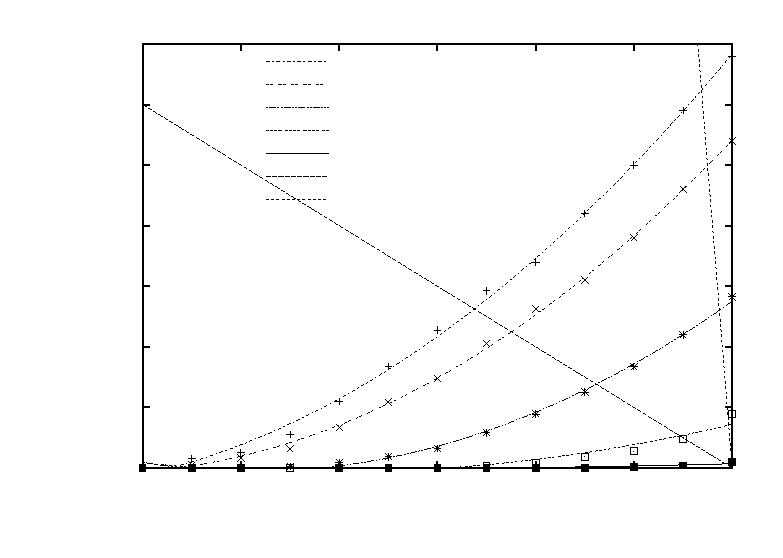
\includegraphics{g1_b}}%
    \gplfronttext
  \end{picture}%
\endgroup

\caption{Graf závislost anodového proudu na anodovém napětí pro různá mřížková napětí.}
\label{g1}
\end{figure}

\subsection{Zesílení}
V zapojení dle obrázku 2 z \cite{text} jsem za stálé konfigurace uvedené v úkolu 2 jsem měřil velikost výstupního napětí 
$U_{vyst}$ na frekvenci $f$ a dle vzorce \ref{A} jsem vypočítal zesílení $A$.
Naměřené hodnoty jsou shrnuty v tabulce \ref{Uvyst} a zesílení $A$ znázorněno v obrázku \ref{g2}.

\begin{table}
$$
\begin{array}{|c||c|c||c|c|}
\hline
R/\Omega &  \multicolumn{2}{|c|}{10^5} & \multicolumn{2}{|c|}{ 5 \cdot 10^3} \\
\hline \hline
f/\mbox{Hz} & U_{vyst}/\mbox{V} &   A   &  U_{vyst}/\mbox{V}    &   A   \\ \hline
30      &    3.4\pm 0.2 &17\pm4     &    2.8\pm 0.2   &14\pm3     \\ \hline
50      &    5.0\pm 0.2 &25\pm5     &    4.4\pm 0.2   &22\pm4     \\ \hline
80      &    6.4\pm 0.2 &32\pm6     &    5.0\pm 0.2   &25\pm5     \\ \hline
100     &    6.6\pm 0.2 &33\pm6     &    5.4\pm 0.2   &27\pm5     \\ \hline
150     &    7.2\pm 0.2 &36\pm6     &    5.8\pm 0.2   &29\pm5     \\ \hline
300     &    7.6\pm 0.2 &38\pm7     &    6.2\pm 0.2   &31\pm6     \\ \hline
500     &    7.8\pm 0.2 &39\pm7     &    6.2\pm 0.2   &31\pm6     \\ \hline
800     &    7.8\pm 0.2 &39\pm7     &    6.2\pm 0.2   &31\pm6     \\ \hline
1000    &    7.8\pm 0.2 &39\pm7     &    6.2\pm 0.2   &31\pm6     \\ \hline
1500    &    7.4\pm 0.2 &37\pm6     &    6.2\pm 0.2   &31\pm6     \\ \hline
3000    &    7.4\pm 0.2 &37\pm6     &    6.2\pm 0.2   &31\pm6     \\ \hline
5000    &    7.2\pm 0.2 &36\pm6     &    6.2\pm 0.2   &31\pm6     \\ \hline
8000    &    6.8\pm 0.2 &34\pm6     &    6.2\pm 0.2   &31\pm6     \\ \hline
10000   &    6.8\pm 0.2 &34\pm6     &    6.2\pm 0.2   &31\pm6     \\ \hline
15000   &    6.2\pm 0.2 &31\pm6     &    6.6\pm 0.2   &33 \pm7    \\ \hline
30000   &    4.8\pm 0.2 &24\pm5     &    6.6\pm 0.2   &33\pm7     \\ \hline
50000   &    3.2\pm 0.2 &16\pm3     &    6.6\pm 0.2   &33\pm7     \\ \hline
80000   &    2.0\pm 0.2 &10\pm3     &    6.6\pm 0.2   &33\pm7     \\ \hline
100000  &    1.6\pm 0.2 &8\pm3     &    6.6\pm 0.2   &33\pm7     \\ \hline
\end{array}
$$
\caption{Tabulka výstupního napětí v závislosti na frekvenci}
\label{Uvyst}
\end{table}

\begin{figure}
% GNUPLOT: LaTeX picture with Postscript
\begingroup
  \makeatletter
  \providecommand\color[2][]{%
    \GenericError{(gnuplot) \space\space\space\@spaces}{%
      Package color not loaded in conjunction with
      terminal option `colourtext'%
    }{See the gnuplot documentation for explanation.%
    }{Either use 'blacktext' in gnuplot or load the package
      color.sty in LaTeX.}%
    \renewcommand\color[2][]{}%
  }%
  \providecommand\includegraphics[2][]{%
    \GenericError{(gnuplot) \space\space\space\@spaces}{%
      Package graphicx or graphics not loaded%
    }{See the gnuplot documentation for explanation.%
    }{The gnuplot epslatex terminal needs graphicx.sty or graphics.sty.}%
    \renewcommand\includegraphics[2][]{}%
  }%
  \providecommand\rotatebox[2]{#2}%
  \@ifundefined{ifGPcolor}{%
    \newif\ifGPcolor
    \GPcolorfalse
  }{}%
  \@ifundefined{ifGPblacktext}{%
    \newif\ifGPblacktext
    \GPblacktexttrue
  }{}%
  % define a \g@addto@macro without @ in the name:
  \let\gplgaddtomacro\g@addto@macro
  % define empty templates for all commands taking text:
  \gdef\gplbacktext{}%
  \gdef\gplfronttext{}%
  \makeatother
  \ifGPblacktext
    % no textcolor at all
    \def\colorrgb#1{}%
    \def\colorgray#1{}%
  \else
    % gray or color?
    \ifGPcolor
      \def\colorrgb#1{\color[rgb]{#1}}%
      \def\colorgray#1{\color[gray]{#1}}%
      \expandafter\def\csname LTw\endcsname{\color{white}}%
      \expandafter\def\csname LTb\endcsname{\color{black}}%
      \expandafter\def\csname LTa\endcsname{\color{black}}%
      \expandafter\def\csname LT0\endcsname{\color[rgb]{1,0,0}}%
      \expandafter\def\csname LT1\endcsname{\color[rgb]{0,1,0}}%
      \expandafter\def\csname LT2\endcsname{\color[rgb]{0,0,1}}%
      \expandafter\def\csname LT3\endcsname{\color[rgb]{1,0,1}}%
      \expandafter\def\csname LT4\endcsname{\color[rgb]{0,1,1}}%
      \expandafter\def\csname LT5\endcsname{\color[rgb]{1,1,0}}%
      \expandafter\def\csname LT6\endcsname{\color[rgb]{0,0,0}}%
      \expandafter\def\csname LT7\endcsname{\color[rgb]{1,0.3,0}}%
      \expandafter\def\csname LT8\endcsname{\color[rgb]{0.5,0.5,0.5}}%
    \else
      % gray
      \def\colorrgb#1{\color{black}}%
      \def\colorgray#1{\color[gray]{#1}}%
      \expandafter\def\csname LTw\endcsname{\color{white}}%
      \expandafter\def\csname LTb\endcsname{\color{black}}%
      \expandafter\def\csname LTa\endcsname{\color{black}}%
      \expandafter\def\csname LT0\endcsname{\color{black}}%
      \expandafter\def\csname LT1\endcsname{\color{black}}%
      \expandafter\def\csname LT2\endcsname{\color{black}}%
      \expandafter\def\csname LT3\endcsname{\color{black}}%
      \expandafter\def\csname LT4\endcsname{\color{black}}%
      \expandafter\def\csname LT5\endcsname{\color{black}}%
      \expandafter\def\csname LT6\endcsname{\color{black}}%
      \expandafter\def\csname LT7\endcsname{\color{black}}%
      \expandafter\def\csname LT8\endcsname{\color{black}}%
    \fi
  \fi
  \setlength{\unitlength}{0.0500bp}%
  \begin{picture}(7200.00,5040.00)%
    \gplgaddtomacro\gplbacktext{%
      \csname LTb\endcsname%
      \put(1078,704){\makebox(0,0)[r]{\strut{} 0}}%
      \put(1078,1286){\makebox(0,0)[r]{\strut{} 100}}%
      \put(1078,1867){\makebox(0,0)[r]{\strut{} 200}}%
      \put(1078,2449){\makebox(0,0)[r]{\strut{} 300}}%
      \put(1078,3030){\makebox(0,0)[r]{\strut{} 400}}%
      \put(1078,3612){\makebox(0,0)[r]{\strut{} 500}}%
      \put(1078,4193){\makebox(0,0)[r]{\strut{} 600}}%
      \put(1078,4775){\makebox(0,0)[r]{\strut{} 700}}%
      \put(1210,484){\makebox(0,0){\strut{}-8}}%
      \put(1917,484){\makebox(0,0){\strut{}-6}}%
      \put(2625,484){\makebox(0,0){\strut{}-4}}%
      \put(3332,484){\makebox(0,0){\strut{}-2}}%
      \put(4040,484){\makebox(0,0){\strut{} 0}}%
      \put(4747,484){\makebox(0,0){\strut{} 2}}%
      \put(5454,484){\makebox(0,0){\strut{} 4}}%
      \put(6162,484){\makebox(0,0){\strut{} 6}}%
      \put(6869,484){\makebox(0,0){\strut{} 8}}%
      \put(308,2739){\rotatebox{-270}{\makebox(0,0){\strut{}$H$/Am$^{-1}$}}}%
      \put(4039,154){\makebox(0,0){\strut{}$x$/cm}}%
    }%
    \gplgaddtomacro\gplfronttext{%
      \csname LTb\endcsname%
      \put(5882,4602){\makebox(0,0)[r]{\strut{}12 cm}}%
      \csname LTb\endcsname%
      \put(5882,4382){\makebox(0,0)[r]{\strut{}16 cm}}%
      \csname LTb\endcsname%
      \put(5882,4162){\makebox(0,0)[r]{\strut{}20 cm}}%
    }%
    \gplbacktext
    \put(0,0){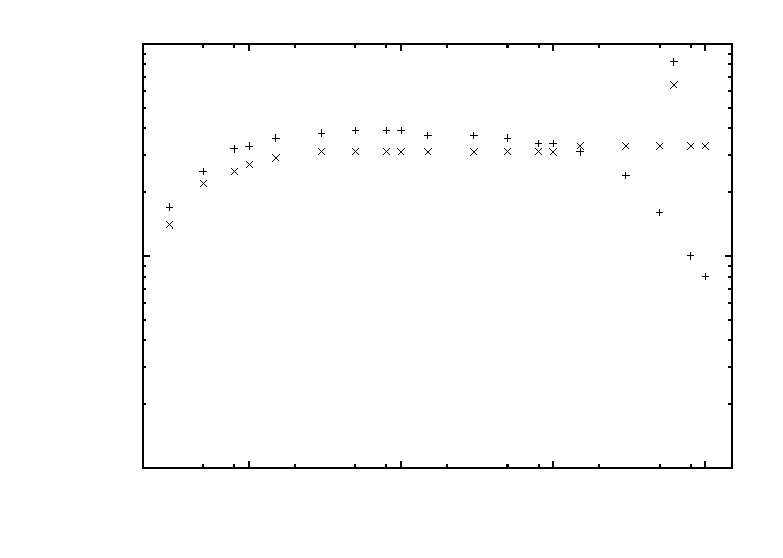
\includegraphics{g2}}%
    \gplfronttext
  \end{picture}%
\endgroup

\caption{Graf závislosti zesílení na vstupní frekvenci pro různé anodové odpory.}
\label{g2}
\end{figure}

Dále jsem nastavil obvod do stavu popsaném v úkolu 3 a měřil velikost výstupního napětí na velikosti anodového odporu. 
Z těchto hodnot jsem následně vypočetl zesílení $A$. Výsledky jsou shrnuty v tabulce \ref{TA}

\begin{table}
$$
\begin{array}{|c|c|c|}
\hline
R_a/\Omega& U_{vyst}/\mbox{V}&  A \\  \hline
5\cdot 10^3&    1.8\pm 0.2&    9\pm2  \\  \hline
6\cdot 10^3&    2.2\pm 0.2&    11\pm3  \\ \hline
7\cdot 10^3&    2.4\pm 0.2&    12\pm3  \\ \hline
8\cdot 10^3&    2.7\pm 0.2&    14\pm3 \\   \hline
9\cdot 10^3&    2.8\pm 0.2&    14\pm3  \\ \hline
10^4&   3.2\pm 0.2&    16\pm3 \\  \hline
2\cdot 10^4&    5\pm 0.2&  25\pm5 \\ \hline
3\cdot 10^4&    6.8\pm 0.2&    34\pm6 \\ \hline
4\cdot 10^4&    7.6\pm 0.2&    38\pm7 \\ \hline
5\cdot 10^4&    8.4\pm 0.2&    42\pm7 \\ \hline
6\cdot 10^4&    8.0 \pm 0.5&    40\pm9 \\ \hline
7\cdot 10^4&    9.0\pm 0.5 &  45\pm9 \\ \hline
8\cdot 10^4&    9.0\pm 0.5& 45\pm9 \\ \hline
9\cdot 10^4&    10.0\pm 0.5&    50\pm10 \\ \hline
10^5&   10.0\pm 0.5&    50\pm10 \\  \hline
\end{array}
$$
\caption{Tabulka velikosti výstupního napětí na velikosti anodového odporu.}
\label{TA}
\end{table}

\begin{figure}
\input{"g3.tex"}
\caption{Graf záislosti zesíleni na velikosti anodového odporu}
\label{g3}
\end{figure}


\eject
\section{Diskuze}

Při proměřování anodových charakteristik triody nebyla přokročena hranice ztráty 0.2~W. Díky přesným přístrojům 
je také chyba malá.

Měření zesílení také vyšlo dle očekávání. Chyba měření je však znatelně větší. Nastavení anodového napětí 
bylo vcelku přesné. Problém však nastal u vstupu. Kolo určující frekvenci proudu podle mě nebylo dostatečně 
přesné a určitě by pomohlo zapojit digitání čítač pro zajištění přesné frekvence. Napětí na zdroji také 
nebylo zcela konstantní. Bylo totíž závislé na frekvenci a i s jemnou korekcí docházelo k jisté chybě. 
Velikost chyby by také pomohlo, kdybych použil u menších hodnot lepší rozsah voltmetru.


\section{Závěr}
\noindent
Změřil jsem anodové charakteristiky triody při různých mřížkových napětích. Výsledky jsou shrnuty v tabulce \ref{Ia} a obrázku \ref{g1},
 kde jsou zakresleny i pracovní body z úkolu 4.\\
Změřil jsem závislost zesílení triody na frekvenci. Výsledky jsou v tabulce \ref{Uvyst} a obrázku \ref{g2}. \\
Změřil jsem závislost zesílení triody na anodovém odporu. Výsledky jsou v tabulce \ref{Ia} na obrázku \ref{g3}.


\eject

\begin{thebibliography}{5}
	\bibitem{text} \textbf{Studijní text na praktikum II} \\http://physics.mff.cuni.cz/vyuka/zfp/txt\_215.pdf (1. 10. 2011)
    \bibitem{chyba} \emph{J. Englich}: \textbf{Zpracování výsldků fyzikálních měření} \\ LS 1999/2000
\end{thebibliography}
\end{document}
